
\documentclass{article}
\usepackage{tikz}
\usepackage{amsmath}
\usetikzlibrary{arrows}
\begin{document}
\begin{title}
\centering

 
\LARGE\textbf{Deriving a Lognormal Stock Price Model}

\bigskip
    

\end{title}
\title{Deriving a Lognormal Stock Price Model}

Assume that stock prices are a stochastic process: $$\{S(t)\}_{t\geq0}$$ The price of t at any time is random. Lets try to answer the question: What is the distribution of these random variables? \\
\section{\textbf{Assumptions:}}


\textbf{A. Efficient Market Hypothesis:} roughly speaking states that the stock price of say t = 10 shouldn't depend on the stock price at time 0, 1, 2, etc. only the instantaneous future. So the stock price at t = 10.0001 should only depend on the stock price at time 10. In other words. This is a Markov assumption that the stock price only depends on the immediate past. 
No one queries the price of a stock in 1932 to figure out the stock price tomorrow - the stock could be bankrupt or could be thriving... we don't know. \\
\\ \textbf{B. Breaking it down into n-steps follows a Normal Distribution:}\\ If the one year returns is $N(0,1)$, then $\frac{1}{n}$ time steps are $N(0,\frac{1}{n})$ as shown by the number line below: 
    \\
\\
\\

        
     \begin{center}
    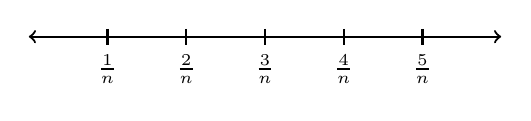
\begin{tikzpicture}
        % Draw number line with arrows on both ends
        \draw[thick, <->] (0,0) -- (6,0) coordinate[midway] (mid);

        % Define tick positions and labels
        \foreach \x in {1,2,3,4,5} {
            \draw[thick] ({\x},0.1) -- ({\x},-0.1); % Tick marks
            \node[below] at ({\x},-0.1) {\small $\frac{\x}{n}$}; % Labels
        }
     
    \end{tikzpicture}
\end{center}
If you break up the year into n equal pieces, all of those pieces must have the same distribution$N(0,\frac{1}{n})$ and be independent of each other. This means that $\sigma\approx\frac{1}{\sqrt{n}}$
\\
\\
\textbf{C. The expected return and volatility do not depend on the price but rather the percentages do (relative price):} If you have 100 shares in the stock and you expect a 10\% return if you have 10,000 shares instead you should reasonably expect the same return of 10\%. Same for volatility. If you own 100 dollars worth of a position that shouldn't change if you own 1000 dollars worth of a position. The volatility shouldn't change based on the scale it's a relative ratio. We can define this mathematically as: 
\\
$$\frac{\Delta s}{s}$$
\newpage
\section{Formulating a Model}
\begin{center}
 $\Delta S = \mu S \Delta t +\sigma S \Delta W$
\\\   

\end{center}

The change in a stock price can be defined as a constant drift (expected return) $\mu$ over time $\Delta t$ and the volatility $\sigma$ times $\Delta W$ where delta W represents the increments of randomness in stock price movements. 
\begin{center}



$\Delta W = \sqrt{\Delta t}$
\end{center}

We know that $\Delta W$ follows a Normal Distribution. According to the Central Limit Theorem, if $\Delta W = W_{t+\Delta t} - W_t \sim N(0, \Delta t)$ the standard deviation is $\sqrt{\Delta t}$. 
\\\
\\\
In continuous time we rewrite the equation as:  
\begin{center}
 $d S = \mu S dt +\sigma S d W$
\\\   

\end{center}

In this context the dW is the differential Brownian Motion. This is our Lognormal model of stock growth. 
\newpage
\section{Why it is Lognormal}
If we consider f(S) = ln(S) and we use Itô's formula: 

\begin{center}
$df = f_t+\mu Sf_s +\frac{1}{2}\sigma^2S^2f_{ss} +\sigma Sf_sdW$
\end{center}
Where $f_t+\mu Sf_s +\frac{1}{2}\sigma^2S^2f_{ss}$ is the deterministic component and $\sigma Sf_sdW$ is the random component 
\\\
Now the derivative of f with respect to S $f_s =\frac{1}{S}$ and $f_{ss} =\frac{-1}{S^2}$ so df satisfies the following Itô: 
\begin{center}

 $ df= f_t +\mu S f_s + \frac{1}{2}\sigma^2S^2f_{ss}$ 
\\\
\\\
$f_t$ can be ignored because there is no t dependence 
\\\
\\\ $\mu Sf_s = \mu S \frac{1}{S} = \mu$
\\\
\\
$\frac{1}{2}\sigma^2S^2f_{ss} =\frac{1}
{2}\sigma^2S^2\frac{-1}{S^2} = -\frac{1}{2}\sigma^2 $
\\\
\\\
$\sigma Sf_sdW = \sigma S\frac{1}{S}dW = \sigma dW$
\\\
\\\
So $df = [\mu -\frac{1}{2}\sigma^2 ]dt + \sigma dW$

\end{center}

Now we know what f is if we integrate the stochastic equation we will get: 
\begin{center}

$ln(\frac{S(t)}{S(0)}) =[\mu -\frac{1}{2}\sigma^2 ]t+  \sigma W(t) $
Therefore: $S(t) = S(0)e^{(\mu  -\frac{1}{2}\sigma ) t+ \sigma W(t)}$
\end{center}
It is an exponential with a normally distributed variable which is why it is called a lognormal distribution. 

\end{document}
